\begin{figure}[htbp]
\centering
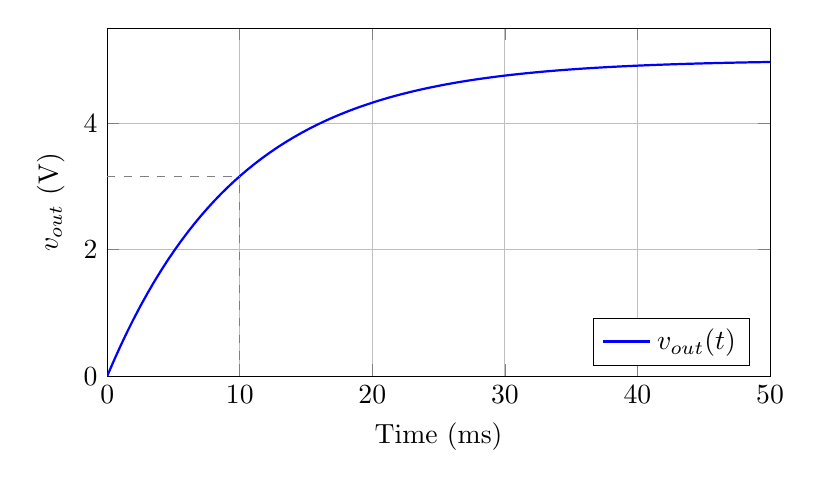
\begin{tikzpicture}
\begin{axis}[
    width=10cm, height=6cm,
    xlabel={Time (ms)},
    ylabel={$v_{\text{out}}$ (V)},
    xmin=0, xmax=50,
    ymin=0, ymax=5.5,
    grid=major,
    legend pos=south east
]
\addplot[blue, thick, domain=0:50, samples=100] {5*(1 - exp(-x/10))};
\addlegendentry{$v_{\text{out}}(t)$}

\draw[dashed, gray] (axis cs:10,0) -- (axis cs:10,3.16);
\draw[dashed, gray] (axis cs:0,3.16) -- (axis cs:10,3.16);
\node[left] at (axis cs:0,3.16) {3.16};
\node[below] at (axis cs:10,0) {$\tau$};
\end{axis}
\end{tikzpicture}
\caption{RC circuit step response.}
\label{fig:rc_step}
\end{figure}
